\documentclass[crop,tikz]{standalone}
\usepackage[subpreambles=true]{standalone}

\usepackage{pgf, tikz}
\usetikzlibrary{shapes.misc}
\usetikzlibrary{decorations.pathreplacing}

\tikzset{cross/.style={cross out, draw=black, minimum size=2*(#1-\pgflinewidth), inner sep=0pt, outer sep=0pt},
%default radius will be 1pt. 
cross/.default={0.25pt},
    point/.style={
    thick,
    draw=black,
    cross out,
    inner sep=0pt,
    minimum width=4pt,
    minimum height=4pt,
    },
}

\begin{document}

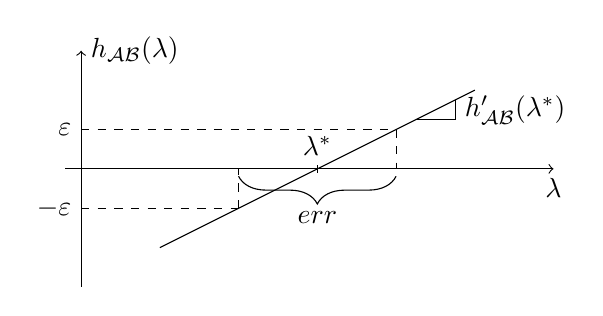
\begin{tikzpicture}
\draw[->] (0,-1.5) -- (0,1.5) node[right]{$h_{\mathcal{A}\mathcal{B}}(\lambda)$};
\draw[->] (-0.2,0) -- (6,0) node[below]{$\lambda$};
\draw (3,-0.05) -- (3,0.05) node[above]{$\lambda^*$};
\draw (1,-1) -- (5,1);
\draw[dashed, thin] (0,0.5) node[left]{$\varepsilon$} -- (4,0.5);
\draw[dashed, thin] (4,0.5) -- (4,0);
\draw[dashed, thin] (0,-0.5) node[left]{$- \varepsilon$} -- (2,-0.5);
\draw[dashed, thin] (2,-0.5) -- (2,0);
\draw (4.25,1.25/2) -- (4.75,1.25/2);
\draw (4.75,1.25/2) -- (4.75,1.75/2) node[midway,right]{$h'_{\mathcal{A}\mathcal{B}}(\lambda^*)$};
\draw [decorate,decoration={brace,amplitude=10pt,mirror},yshift=3pt] (2,-0.2) -- (4,-0.2) node [black,midway,yshift=-15pt] {$err$};
\end{tikzpicture}

\end{document}